\chapter{Inleiding}
\begin{chapquote}[30pt]{Douglas Adams, \textit{Hitchiker's Guide to the Galaxy}}
Now, [a Babel Fish\footnote{The Babel fish is small, yellow and leech-like, and probably the oddest thing in the Universe. It feeds on brainwave energy received not from its own carrier but from those around it. It absorbs all unconscious mental frequencies from this brainwave energy to nourish itself with. It then excretes into the mind of its carrier a telepathic matrix formed by combining the conscious thought frequencies with the nerve signals picked up from the speech centres of the brain which has supplied them. The practical upshot of all this is that if you stick a Babel fish in your ear you can instantly understand anything said to you in any form of language. The speech patterns you actually hear decode the brainwave matrix which has been fed into your mind by your Babel fish.\citep{adams}}%
] is such a bizarrely improbable coincidence that anything so mind-bogglingly useful could have evolved purely by chance that some have chosen to see it as the final proof of the NON-existence of God. The argument goes something like this:\\[2.5pt]
\enquote{I refuse to prove that I exist,} says God, \enquote{for proof denies faith, and without faith I am nothing.}\\[2.5pt]
\enquote{But,} says Man, \enquote{the Babel fish is a dead giveaway, isn't it? It could not have evolved by chance. It proves that You exist, and so therefore, by Your own arguments, You don't. QED.}\\[2.5pt]
\enquote{Oh dear,} says God, \enquote{I hadn't thought of that,} and promptly vanishes in a puff of logic.\\[2.5pt]
\enquote{Oh, that was easy,} says Man, and for an encore goes on to prove that black is white and gets himself killed on the next zebra crossing.
\end{chapquote}

Er zijn diverse redenen waarom ICT'ers logica zouden moeten leren. Logica is allereerst historisch gezien de basis van de moderne informatica, immers zowel het werk van Church als dat van Turing (zie terzijde \ref{as:frege}) komt voort uit het beslisbaarheidsprobleem van eerste-orde logica. Moderne aanpakken in de informatica, vooral op het gebied van de \emph{kunstmatige intelligentie}, genereren een als maar groeiende interesse in logica, door het voornemen om immer meer te automatiseren en de noodzaak tot het bewijzen van de correctheid van computer programma's. 

In de basis is logica een middel tot het formaliseren van taal en het redeneren. Informatica heeft in essentie hetzelfde probleem en verder reikende doelen; na het formaliseren probeert de informatica die formalisatie uit te drukken om er zodoende mechanismen van te maken die de gevonden regels navolgen. Dit heeft ervoor gezorgd dat logica nu meer een onderdeel gezien wordt van de informatica dan van de wiskunde. De groei van beide gebieden is echter nauw verbonden; door vooruitgang in informatica worden er nieuwe idee\"en geopperd  voor logische analyse, en deze logisch idee\"en bevorderen op hun beurt ontwikkelingen in de informatica.

\begin{aside}[Van logica tot informatica, een korte geschiedenis]\label{as:frege}
Halverwege vorige eeuw was het George Boole die de wiskundige basis legde voor computer hardware en propositielogica. Zijn werk was echter gebaseerd op dat van de Duitse filosoof en wiskundige Gottlob Frege (eind 19e eeuw). Frege had zichzelf als doel gesteld om alle wiskundige principes af te leiden vanuit de logisch principes. Hiermee trachtte hij een systeem te ontwikkelen van \enquote{puur redeneren} (naar een idee van de 17e eeuwse Gottfried Wilhelm Leibniz), met slechts enkele zelf-evidente basisbeginselen zoals die van verzamelingen. 


  \begin{marginfigure}
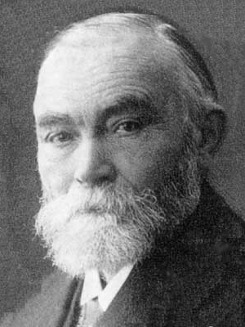
\includegraphics[width=0.6\textwidth]{frege.png}\\
    Gottlob Frege {\scriptsize\emph (Image by Wikipedia)}\\[3mm]
  \end{marginfigure}

  \begin{marginfigure}
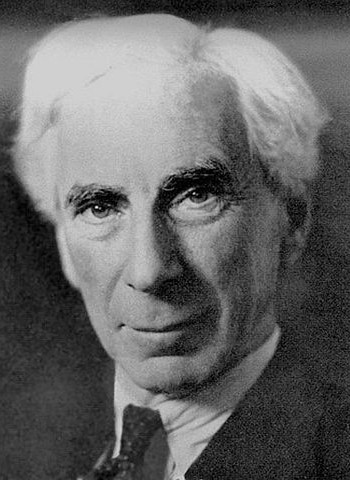
\includegraphics[width=0.6\textwidth]{russel.jpg}\\
    Bertrand Russell {\scriptsize\emph (Image by Wikipedia)}\\[3mm]
  \end{marginfigure}

\hspace{15pt}Door deze ontwikkeling introduceerde hij een nieuwe notatie en taal die de basis vormde van zijn werk en ten grondslag ligt aan de predikaatlogica die wij in deze reader zullen behandelen (zie hoofdstuk \ref{ch:predicaten}). Tot de aanpassingen van Boole en Frege was de logica, als mechanisme tot het onderzoeken en uitdrukken van het menselijk redeneren, niet verandert sinds zijn introductie door Aristoteles (circa 300 BC.).

\hspace{15pt}Frege's enorme werk werd verwoestend bekritiseerd door Bertrand Russell, die een fundamentele fout had gevonden in de zelf-evidente basis van Frege's werk (zie terzijde \ref{as:russel:paradox}). Echter werkte Russel vervolgens mee aan het repareren van deze kritieke fout, en verspreidde daarmee de idee\"en onder de Engelse wiskundigen (waaronder Boole, en later Turing en Church).
\footnotetext{Vrij naar `Logicomix -- An Epic Search for Truth', \citet{logicomix}.}
\end{aside}

\section{Metataal}\label{sec:metataal}
In deze reader behandelen wat bekend staat als `wiskundige logica', `symbolische logica' of `formele logica'\footnote{In tegenstelling tot `filosofische logica'.} Dat betekent dat we gebruik zullen maken van bekende wiskundige methoden om te onderzoeken wat logica inhoudt. Om deze context wat duidelijker te maken trekken we hier de vergelijking met een typische introductiecursus programmeren.

Een programmeercursus leert je niet alleen welke constructen uit de taal je kan gebruiken om bepaalde gevolgen te behalen als je het programma uitvoert, maar het leert je ook het verschil tussen de taal waarin je de programma's schrijft en de betekenis van die statements in termen van het effect ervan als ze worden uitgevoerd door de computer.
Als het een goede cursus zou zijn, dan zou ze je ook leren na te denken over programma's, bijvoorbeeld om in te zien dat twee verschillend lijkende programma's feitelijk hetzelfde zijn (of hetzelfde bereiken).

Logica is de studie van formele (symbolische) systemen van het redeneren en het bepalen van betekenis. Ze is vergelijkbaar met een introductie programmeren omdat beiden een analyse van formele systemen omvat als ook een analyse van betekenis (semantiek). Echter, in Logica bestudeer je veel meer diverse formele systemen dan in de informatica, zodat je logica niet alleen gebruikt als wiskundig middel voor de analyse, maar ook als fundament voor de wiskunde zelf. Dit zou de nodige alarmbellen moeten doen rinkelen, omdat we al hadden gezegd dat we wiskunde zouden gebruiken om Logica te bestuderen, dus we hebben te maken met een cirkelredenering (of \enquote{zelf-referentie}).

In de logica bestrijden we deze zelf-referentie door een duidelijk onderscheid te maken tussen de logica die we \underline{bestuderen} en de logica die we gebruiken om \underline{mee} te bestuderen. De logica die bestudeert wordt drukken we uit in een specifieke taal (de \emph{objecttaal}), terwijl de analyse van deze logica en taal uitgevoerd wordt in een andere taal (de \emph{metataal}).

Dit idee zou niet geheel vreemd voor je moeten zijn. Immers als je bijvoorbeeld Latijn zou bestuderen, zijn uitspraken in het Latijn in de objecttaal, terwijl de discussies die je voert over deze uitspraken in het Nederlands (de metataal). In de wiskunde is het niet anders (bijv., in calculus, verzamelingenleer, grafentheorie, etc.), maar ook in de informatica. In deze laatste is de objecttaal de taal waarin we programmeren, zoals Python, Java, Lisp, Miranda, en de metataal wederom Nederlands, mogelijk uitgebreid met wat toepasselijke wiskundige en informatica specifieke termen.

\begin{example}\mbox{}\\
Beschouw de volgende uitdrukking:
\begin{quote}\begin{texttt}times 0 do print * od = do\_nothing
\end{texttt}\end{quote}
\end{example}
Dit is, wezenlijk, een uitspraak in de metataal over de equivalentie van twee uitdrukkingen in een of andere programmeertaal. Wellicht had je het zelf ook al bedacht, maar het is bijzonder lastig om exact te bepalen welke symbolen tot de objecttaal en welke tot de metataal behoren. Figuur \ref{fig:metataal} geeft hierover verheldering.
\begin{figure}[h]
\begin{center}
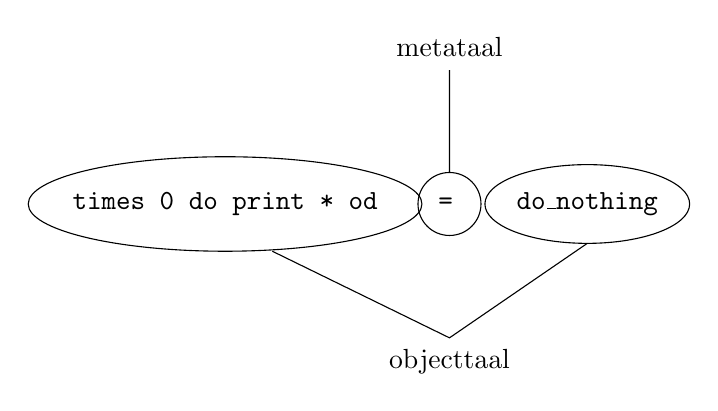
\begin{tikzpicture}
\node at (-0.1,0) {\tt times 0 do print * od};
\node at (2.7,0) {\tt =};
\node at (4.5,0) {\tt do\_nothing};
\draw (-0.1,0) ellipse (2.5cm and .6cm);
\draw (2.75,0) circle (.4cm);
\draw (4.5,0) ellipse (1.3cm and .5cm);
\node at (2.75, 2) {metataal};
\node at (2.75, -2) {objecttaal};
\draw (2.75,1.7) to (2.75,.4) (.5,-.6) to (2.75,-1.7) to (4.5,-.5);
\end{tikzpicture}
\caption{Onderscheid objecttaal en metataal.}\label{fig:metataal}
\end{center}
\end{figure}

Om correct te kunnen bepalen welke elementen tot welke taal behoren, is het noodzakelijk om een goede definitie te hebben van de objecttaal. Dit is het eerst dat we zullen doen in hoofdstuk \ref{ch:proposities}.

\section{Formalisatie}
Het proces van het opstellen van een objecttaal en het vaststellen van regels om deze te kunnen manipuleren noemen we \emph{formaliseren}. Het doel hiervan is om duidelijkheid te verkrijgen en fouten (misvattingen) te vermijden.

Een tweede, even belangrijke stap van het formaliseren is dat het formaliseren ons de mogelijkheid biedt om objecten te manipuleren zonder te hoeven begrijpen wat we precies aan het doen zijn. Dit klinkt als een stap achteruit, maar laten we een voorbeeld beschouwen: de rekenkunde volgt uit de formalisering van het tellen. Hierdoor hebben we nu regels die we kunnen volgen om getallen correct bij elkaar op te tellen zonder exact te weten wat de getallen zijn of wat optellen is.

De kracht van formaliseren is dan dat als er eenmaal geformaliseerd is, een gebied van interesse bewerkt kan worden zonder dat er begrip voor benodigd is. Zolang er goed is geformaliseerd en de gevonden regels strikt worden nageleefd, is begrip (intelligentie?) niet benodigd voor het uitvoeren van een taak. Zonder hier nu in een diepe filosofische discussie te belanden, hebben we hier zojuist de basis van machine intelligentie verklaard: computers kunnen, zonder begrip van de wereld, intelligente dingen doen, mits ze de juiste formalisaties krijgen aangereikt (d.w.z. wiskunde, logica, etc.) om die intelligente taken te kunnen volbrengen. Het is dus ook van dermate belang dat een AI'er bedreven is in de kunst van het formaliseren.

\section{Terminologie}
Tot slot, voor deze inleiding, rest ons nog de bespreking van enige terminologie die je in deze reader veelvuldig zal tegenkomen. Begrip van deze terminologie is essentieel voor het begrijpen van de aangeboden materie.

Belangrijke beweringen waarvoor een bewijs bestaat, wordt vaak een \textit{stelling} genoemd (Engels: \textit{theorem}). Een iets minder belangrijke bewering waarvoor een bewijs bestaat, wordt wel een \textit{propositie} genoemd (Engels: \textit{proposition}). Een bewering met een bewijs waarvan het belang niet op zich zelf staat, maar voornamelijk dient als hulpresultaat om een stelling te bewijzen, heet een \textit{lemma}. Een gevolg van een stelling wordt wel \textit{corollarium} genoemd (Engels: \textit{corrolary}). Het precies vastleggen van de betekenis van een nieuw begrip heet een \textit{definitie}. %Een fundamentele bewering die je niet bewijst maar als uitgangspunt hanteert heet een \textit{axioma}.

Bij een bewijs is het handig om te zien waar het begint en eindigt. Meestal begint het met het woord \textit{bewijs} (Engels: \textit{proof}, en eindigt het met een blokje $\square$). In sommige teksten wordt een bewijs afgesloten met de afkorting Q.E.D.. Dit staat voor \textit{quod erat demonstrandum}, hetgeen Latijn is voor "hetgeen bewezen moest worden". In dit dictaat hanteren wij een zwart blokje: $\blacksquare$.

Een bewering waarvan je verwacht dat die waar is, maar waarvoor geen bewijs gevonden is, heet een \textit{vermoeden} (Engels: \textit{conjecture}). Het is verbazend dat er veel eenvoudig te formuleren beweringen bestaan waarvan de juistheid wel vermoed wordt, en er is dan ook nooit een tegenvoorbeeld voor gevonden, maar waarvoor na uitgebreide inspanningen ook nog nooit een bewijs voor is gevonden.

  \begin{marginfigure}
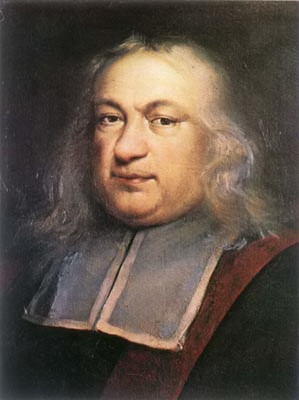
\includegraphics[width=0.6\textwidth]{Pierre_de_Fermat.jpg}\\
    Pierre de Fermat {\scriptsize\emph (Image by Wikipedia)}\\[3mm]
  \end{marginfigure}

\begin{aside}[Stelling van Fermat]\textbf{}\\[2.5pt]
Het komt ook wel voor dat dergelijke vermoedens toch nog bewezen worden. Een frappant voorbeeld hiervoor is de \textit{laatste stelling van Fermat}, rond 1637 door Fermat geformuleerd: \enquote{er bestaan geen gehele getallen $n>2$ en $a,b,c,>0$ waarvoor $a^n+b^n=c^n$}. Hoewel Fermat zelf beweerde hiervoor een wonderbaarlijk bewijs te hebben gevonden dat helaas te groot was om in de kantlijn op te nemen, is dat `bewijs' niet bewaard gebleven en is deze bewering honderden jaren een vermoeden geweest. Tot 1993: toen gaf Andrew Wiles hiervan een bewijs, dat compact opgeschreven enige honderden pagina's besloeg, exclusief de bewijzen van de vele gebruikte veelal zeer diepe al eerder bekende stellingen.
\end{aside}
